\documentclass[10pt,a4paper,twocolumn]{article}

\usepackage[top=0.6in]{geometry}

%for links
%\usepackage[hidelinks]{hyperref}
\usepackage{hyperref}

%for bilbiography
\usepackage{natbib}

%for images
\usepackage{graphicx}
\usepackage{caption}
\usepackage{subcaption}

\author{Dionisio Perez-Mavrogenis}
\title{Firmware Protection and Attacks Against the ATMega Microcontroller Series}
\date{\today}

\begin{document}
	\maketitle
	
\section*{\emph{Abstract}}
	\textbf{\emph{The most abstract abstract of some abstracts, full of abstractions.}}
	

\section{Introduction}
	This paper will present an overview of the current attacks and methods of tampering with Intellectual Property (IP) in MicroController Units (MCUs). In this context IP does not solely refer to the firmware running on the MCU but it includes information that could be obtained from that code, i.e. secrets or proprietary algorithms that help a manufacturer achieve higher performance over their competitors.
	
	Tampering (or theft) detection and prevention of the firmware of a MCU is a popular problem with active research, as solving it would benefit a lot of parties (including the government and the military), as MCUs are used in areas spanning from consumer electronics to missile guiding systems.
	
	A distinction between ordinary and secure microcontrollers should be made\citep{website:scorobogatov_breaking_copy_protection} and, due to the sophistication in the protective mechanisms and the attack vectors, a broad classification of attackers as\cite{anderson:cautionary_note}:
		\begin{itemize}
			\item \textbf{Home Hackers} Clever and curious people with a very limited budget, perhaps with some degree of knowledge and no malicious intent, but with no time-limit.\\
			\item \textbf{Semi-Professional Crackers} Professionals skilled on electronics with access to specialised equipment and resources. Their funding might be limited, malicious intent is unclear and they might be constrained in their time allowance.\\
			\item \textbf{Funded Organisations} Organisations with access to MCU manufacturing equipment. Their funding is usually unconstrained, there usually exists malicious intent and their time schedule is usually tight.
		\end{itemize}
	
	Firmware tampering or theft has a number of consequences. The most obvious consequence is an attacker downloading the code from a MCU and flashing it onto a MCU that they sell, effectively avoiding development and testing costs but still offering the same product as other manufacturers(\cite{tech:aes_bls}). A less obvious, but perhaps more important, case is the case of back-dooring\footnote{The act of adding code to a system without the user's knowledge or approval, usually to accomplish nefarious tasks.} a MCU by re-flashing on it a modified version of the firmware with coded added by the attacker in order to accomplish their malicious intents, which could have disastrous consequences if these MCUs were used for military or other sensitive operations. 

	\subsection{Objectives}
	The aims of this paper are to review the possible attacks against the ATmega series of MCUs and provide possible countermeasures or possible methods of hardening a system. 
	
	Section \ref{sec:atmega_overview} will provide an overview of the ATmega series of AVRs and explain the most important hardware architecture aspects and protection mechanisms they offer. 
	
	Section \ref{sec:curr_attacks} will give a (brief) overview of the current attack techniques used to override currently implemented protection mechanisms, an overview of whom is given in Section \ref{sec:defenses}. 
	
	In section \ref{sec:attacking_mega} the current attacks will be related to the ATmega, by presenting the attack vectors in more detail as well as providing references to relevant work. Section \ref{sec:conclusion} will conclude the paper with a discussion on the usefulness of hardening the ATmega, contrasting that with using a MCU that is designed to be secure.
	
\section{The AVR MCU Series}
\label{sec:atmega_overview}

	The Atmel AVR series is an enhanced-RISC MCU family that consists of the ATtiny, ATmega and ATxmega sub-categories and derivatives of the above, including 32-bit AVRs and application specific FPGAs\footnote{info:\href{http://www.atmel.com/products/microcontrollers/avr/default.aspx}{AVR family link}}. The models have varying degrees of hardware capabilities and large operating voltage windows in order to accommodate demand and integrate well with peripherals\footnote{info:\href{https://www.newbiehack.com/MicrocontrollersAlternativePowerSources.aspx}{https://www.newbiehack.com}}\footnote{info:\href{http://www.atmel.com/v2PFResults.aspx}{http://www.atmel.com/v2PFResults.aspx}}.
	
	Developing software for an AVR is easy as the AVRs benefit from the free \texttt{avr-libc} high-performance C run-time library(optimised for the AVR RISC architecture), the \texttt{avr-gcc} and \texttt{avr-gdb} compiler and debugger(both based on very popular and high quality GNU software tools), the \texttt{avrdude} programming software(or Atmel's proprietary \texttt{AVRStudio}) and \texttt{Simulavr} simulator software. Additionally, Atmel provides proprietary APIs for interacting with the AVR and the developers can choose from a wide variety of programmer units available for working with the AVRs\cite{book:practical_avr}.
	
	\subsection{ATMega Architecture and Features}				

	\subsubsection{Important Feature Overview}
	The ATmega series of MCUs is a relatively large family of MCUs and the focus of this paper is on the ATmega644 and ATmega1284. The only differences between then 1284 and the 644 is that the 1284 has got more memory available and an hardware extra timer. A summary of (some) of the features of the two units is give in Table \ref{table:avr_specs}\citep{atmega_manual}. 
	
	Both MCUs are an enhanced-RISC Harvard architecture 8-bit CPU. Figure \ref{fig:architectures} shows the conceptual difference between a Von Neuman (most modern PCs) and a Harvard architecture, where the key distinction lies in the separation of application code and program data into different memory sections (Harvard) and tasking the CPU with distinguishing between code and data that lives in the same memory region (Von Neuman). The 644/1284 implement a Harvard architecture for both power and computational efficiency, being designed to access more than one registers simultaneously (due to the physical wiring of the CPU), enabling them to execute an instruction per cycle. Their operating voltages can vary between 1.8V and 5.5V (maximum operating frequency 20 MHz).
	
	\subsubsection{Memory Organisation}
	The 644/1284 are equipped with an EEPROM, flash memory, SRAM, a large number of general purpose registers and a large number of I/O registers (in order to be able to perform I/O) and all memory (including I/O memory mapped images) is linear, i.e. it follows the flat memory model.
	
	The flash memory is separated into two regions, the bootloader section and application code section. The boundary between the two sections can be configured by programming the appropriate fuses, and the page size can also be configured that way as well. Both sections hold code, however code residing in the bootloader section can execute a special instruction (\texttt{SPM}\footnote{\texttt{SPM} = Store Program Code}) which allows the bootloader code to write to \textit{any} section in the flash memory and hence possibly modify itself(designed for purposes such as firmware upgrades). The bootloader code can be triggered by a direct jump from the application section or by programming the reset vector via the reset fuse to point to the appropriate section of the bootloader code. 
	
	The EEPROM is memory for data that needs to persist between reboots of the MCU and hence it is (widely) used to hold configuration variables and other non-temporary preferences the application code (or the bootloader) may need, having an average lifespan is 100,000 write cycles per page. 
	
	The SRAM is volatile storage and is used as the stack and heap for the software (either application code or bootloader code) as well as for storing the Register File (i.e. the 32 GP registers) I/O and Extended I/O Memory. The reserved register locations exist in order to support the use of peripheral units as well as hold program status information (e.g. the Stack Pointer can be found in one of the GP registers).Figure \ref{fig:stack} gives an overview of the SRAM hierarchy, which is slightly different (in terms of region sizes) for the 644 and the 1284 as the 1284 offers more SRAM.
	
	\begin{figure}
		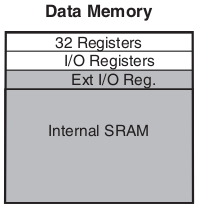
\includegraphics[scale=0.7]{img/stack.png}
		\caption{SRAM layout for the ATmega 644 and 1284. \textbf{Source}:\protect\citep{atmega_manual}.}
		\label{fig:stack}		
	\end{figure}
	
\begin{figure*}
	\begin{subfigure}{0.5\textwidth}
		\center
		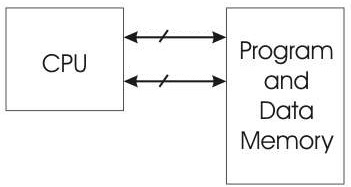
\includegraphics[scale=0.5]{img/von_neuman_arch.jpg}
		\caption{Schematic of a Von Neuman architecture.}
		\label{fig:VN_arch}
	\end{subfigure} 
	~
	\begin{subfigure}{0.5\textwidth}
		\center
		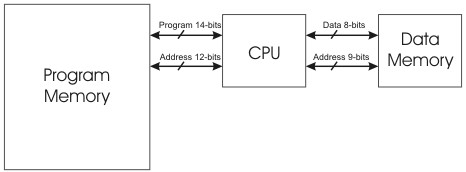
\includegraphics[scale=0.5]{img/harvard_arch.jpeg}
		\caption{Schematic of a Harvard architecture.}
		\label{fig:H_arch}
	\end{subfigure}
	\caption{A comparison of different machine architectures. \textbf{Source}:\protect\citep{website:mcu_primer}.}
	\label{fig:architectures}
\end{figure*}	
		
	\begin{table*}
		\begin{tabular}{| c | p{2cm} | p{1.5cm} | p{3cm} | p{2.8cm} | c | p{1.9cm} |}
		\textbf{Model} & \textbf{EEPROM (Kb)} & \textbf{SRAM (Kb)} & \textbf{Programmable Flash(Kb)} & \textbf{SPI Port} & \textbf{JTAG Interface}\\
		ATmega644 & 2 & 4 & 64 & Yes & Yes\\
		ATmega1284 & 4 & 16 & 128 & Yes & Yes \\
		
		
		\end{tabular}
	\caption{Specification overview for the AVR ATmega644 and ATmega1284}
	\label{table:avr_specs}
	\end{table*}
	
	\subsection{ATMega Security Features}
	
	The AVR ATmega644/1284, even though not meant to be secure hardware modules, posses certain security features. In particular, each board provides six Lock bits (which can be programmed or unprogrammed) and which are responsible for controlling or preventing different memory portions of the board to be modified or read by the other parts (e.g. prevent code executing from the bootloader section to read/write the application code section via the \texttt{SPM} instruction). The prevention however is not permanent, as that would limit the usefulness of the MCU and therefore one has the option to bring these lock bits back to State 1 (i.e. unprogrammed, having no protection scheme enabled) by issuing a Chip Erase command, which has the effect of completely erasing the Flash, EEPROM and Lock bits.
	
	The erasing is performed with the sequence of events presented above and this is important, as one does not want to remove the access protection before removing all sensitive data and hence the Lock bits are set to 1 only after the whole program memory has been erased. Even though the flash memory has an average lifespan of 10,000 write cycles (as well as programming being relatively expensive as an operation) this approach makes sense as the ultimate goal is to preserve the intellectual property on the board rather than the board itself.
	
	\begin{table*}
		\center
		\begin{tabular}{| c | c | c | c |}
			\hline
			\textbf{Lock Bit Byte} & \textbf{Bit Number} & \textbf{Description} & \textbf{Default Value}\\
			\hline \hline
			BLB12 & 5 & Boot Lock Bit & 1\\
			BLB11 & 4 & Boot Lock Bit & 1\\
			BLB02 & 3 & Boot Lock Bit & 1\\
			BLB01 & 2 & Boot Lock Bit & 1\\
			LB2 & 2 & Lock Bit & 1 \\
			LB1 & 1 & Lock Bit & 1 \\
			\hline
		\end{tabular}
		\caption{Security lock bits offered by the ATmega644 and ATmega1284.}
		\label{table:lock_bits}
	\end{table*}
	
Table \ref{table:lock_bits}	 provides an outline of the available Lock bits provided by the ATmega series. The functionality of the BLB1 group is to control access and modification of the bootloader section, group BLB0 bits control access to the application code section and group LB bits are responsible for controlling modifications on the EEPROM and Flash.A detailed explanation of their functionality and how to use them is given in \citep{atmega_manual}.
	
\section{Attacks on Hardware}
\label{sec:curr_attacks}
A distinction between \emph{passive} and \emph{active} attacks should be made. In the former the attacker simply monitors the chip's normal operation and tries to infer the input-output mapping whereas in the latter case the attacker actively manipulates either the chip or its operating environment with the aim of obtaining insight on the chips inner workings. 

Attacks on MCUs attempt to recover key material from either the flash or the EEPROM and do not need to necessarily attack the hardware itself but can leverage flaws in algorithmic design and protocol failures or inter-component communication\citep{anderson:cautionary_note}\citep{kocher:DPA}.

obtain information by corrupting the memory or exploiting memory remanence features\citep{anderson:tamper_resistance}

		apparently sergei has cracked them already \cite{website:scorobogatov_breaking_copy_protection}
	mention attacks may be passive(observing input-$>$output mapping) or active (tamper with the aforementioned mapping in some useful way)
	\subsection{Non-Invasive Attacks}
	SPA-DPA
	\subsection{Semi-Invasive Attacks}
	some sort of fault injection?
		all memory types are linear( as well as memory mapped IO) - related to memory scanning attacks by glitching and power faults (stop making call or jump instructions)
	\subsection{Invasive Attacks}
	Microprobing
	overview of attack categories [each one to the category that it corresponds above]
	\begin{itemize}
		\item microprobing \\
		\item side-channel attacks \\
		\item software attacks (exploit communication protocols or crypto implementation and such) \\
		\item reverse engineering of hardware\\
		\item fault generation (power/clock glitches ) \\
	\end{itemize}
	
	* for each category discuss budget/tools/skillset/time required\\

\section{Countermeasures to known attacks}
\label{sec:defenses}
	\begin{itemize}
	\item overview of most popular techniques \\
	\item benefits and how they improve the situation/approach the problem
	\item added cost for this investment (in terms of hardware and money, transparency to the developers, runtime overhead etc)\\
	\end{itemize}
	
	perhaps review some popular secure chips ??	
	
	

\section{Attacking The ATmega}
\label{sec:attacking_mega}

The ATmega is a typical MCU that is suseptible to a successful attack by the \textbf{Home-Hacker} class of attackers due to its weak protective mechanisms. While there is a way to deliver firmware updates to the MCU securely(\citep{tech:aes_bls}), it will be demonstrated that keeping the firmware secure on the device is impossible.

	\subsection{Motivation}
	
	\subsection{Attack Overview}
		* feasible? 
		* added cost (in terms of \$\$, extra hardware and software implementation penalties/overhead)
	

\section{Evaluation}
\label{sec:conclusion}

No system is unbreakable and one can only harden their system enough to make the effort of breaking it unbearable to those they wish to protect against\citep{anderson:cautionary_note}\cite{website:scorobogatov_breaking_copy_protection}. AES bootloader\citep{tech:aes_bls},

	not sure if the subsections are needed here
	\subsection{Securing the mega}
		paragraph talking about why it's not a good idea to salvage the mega.
	\subsection{Attacks and Solutions overview}
	\subsection{Conclusions}
	
	\bibliographystyle{plain}
	\bibliography{irp_report}	
	
\end{document}
